\chapter{研究现状综述}\label{chap:relatedwork}

% 2.1 引言
\section{引言}
% 任务背景
% 可以介绍统计机器翻译到神经机器翻译的变革,带来了哪些影响,例如在多模态融合等方面的影响
机器翻译是一种利用计算机算法将一种语言翻译到另一种语言的技术。从统计机器翻译时代,到神经机器翻译时代,机器翻译相关技术一直作为行业的风向标引领着整个自然语言处理领域的发展。其基础模型从做到打破语言壁垒突破至跨越模态整合,能够在计算机视觉、语音信号处理以及多模态信息融合等领域都得到广泛的应用。
% 任务起源
% 可以提到机器翻译的缺陷,比如歧义、信息不充足等问题试图通过外源信息来解决
多模态机器翻译就是一种在机器翻译的基础上,融合图像信息、语音信息或者文档上下文信息的一类方法。这些引入的外源信息,在理论上具有解决歧义词、转录错误以及指代不明等问题的意义。

% 任务形式
% 讲讲与机器翻译的区别、如何将其分为了两大类。
融合图片信息的神经机器翻译是多模态神经机器翻译方法的一个分支,是一种将图片作为外源辅助信息输入到神经机器翻译模型中,以提升翻译准确率为目的的一类方法。因此,与常规的神经机器翻译相似的是,相关研究所使用的语料同样需要平行翻译句对的形式,区别在于增加了与文本内容高度相关的图片输入。根据图片信息的作用方式,可以将相关方法分为图片信息辅助式、图片信息增强式、图片搜索式以及基于无监督的方法。本章首先将简要介绍神经机器翻译的发展过程,以及用于对图片进行预处理以及特征提取的计算机视觉基础模型,然后按照图片信息辅助式、图片信息增强式、图片搜索式和基于无监督的方法的分类,分别介绍融合图片信息的神经机器翻译如何随着神经机器翻译的发展而进行改进与进化。

% 2.2 神经机器翻译
\section{神经机器翻译模型}
在融合图片信息的机器翻译任务中,平行翻译句对的原文与译文之间一般具有很强的对齐关系,而图片主要起到补充信息的作用。因此,该任务所使用的模型多数是以NMT的模型作为基础框架,视觉特征作为模型的额外输入。本节将介绍MMT在模型设计发展过程中所应用到的NMT基础模型框架,这其中包含:基于循环神经网络(Recurrent Neural Network,RNN)方法的NMT模型、增加注意力机制的基于RNN的NMT模型以及基于自注意力机制的Transformer。另外,还有基于卷积神经网络(Convolutional Neural Networks,CNN)的NMT模型\cite{6_DBLP:journals/corr/GehringAGYD17},但其很快被自注意力机制取代,也没有在MMT任务上的应用,因此本节忽略这部分内容的介绍。

\subsection{循环神经网络}
神经机器翻译是一种序列到序列的生成任务,其源端序列与目标端序列的长度往往是不同的。因此,编码器-解码器结构成为了神经机器翻译的常用模型框架。编码器和解码器分别用于编码源端序列和解码到目标端序列。循环神经网络就是一种用于解决序列建模的一类方法。图1为基于循环神经网络的神经机器翻译(RNN-based NMT,RNMT)框架。编码器将不定长的源语言句子编码为单个固定维度的隐层向量,该隐层向量可作为整个句子语义的特征表示。解码器负责根据该特征表示生成目标语言句子。形式化地,给定待翻译的源语言句子$X=\{x_1,x_2,…,x_n\}$,在编码端首先需要将$X$中的词转化为词向量$E=\{\boldsymbol{e}_1,\boldsymbol{e}_2,…,\boldsymbol{e}_n\}$,其中:
\begin{equation}
    \boldsymbol{e}_i=\mathrm{Emb}(x_i)
\end{equation}

源语言句子中的每个词$x_i$均有一个对应的词向量表示$\boldsymbol{e}_i$。然后编码器按照句子中词的顺序将句子编码到一个隐层状态序列$\overrightarrow{\boldsymbol{H}}={\overrightarrow{\boldsymbol{h}}_1,\overrightarrow{\boldsymbol{h}}_2,…,\overrightarrow{\boldsymbol{h}}_n}$,其中,$\overrightarrow{\boldsymbol{h}}_i$中编码了输入序列中前$i$项的信息,即:
\begin{equation}
    \overrightarrow{\boldsymbol{h}}_i=\mathrm{RNN}(\overrightarrow{\boldsymbol{h}}_{i-1},\boldsymbol{e}_i)
\end{equation}
为了使每个位置的编码结果融合到整个输入序列的信息,可采用双向编码器将句子$X$同时编码到$\overrightarrow{\boldsymbol{H}}$和$\overleftarrow{\boldsymbol{H}}$,其中,$\overleftarrow{\boldsymbol{H}}=\{\overleftarrow{\boldsymbol{h}}_1,\overleftarrow{\boldsymbol{h}}_2,…,\overleftarrow{\boldsymbol{h}}_n\}$为$X$的逆序编码结果,即:
\begin{equation}
    \overleftarrow{\boldsymbol{h}}_i=\mathrm{RNN}(\overleftarrow{\boldsymbol{h}}_{i+1},\boldsymbol{e}_i)
\end{equation}
将$\overrightarrow{\boldsymbol{H}}$和$\overleftarrow{\boldsymbol{H}}$拼接得到$\boldsymbol{H}=\{\boldsymbol{h}_1,\boldsymbol{h}_2,\cdots,\boldsymbol{h}_n\}$, 其中:
\begin{equation}
    \boldsymbol{h}_i=[\overrightarrow{\boldsymbol{h}}_i;\overleftarrow{\boldsymbol{h}}_i]
\end{equation}

RNMT的解码器同样采用循环神经网络来生成目标语言文本。该生成翻译的过程是自回归的,即在时刻$t$,解码器需要根据$0$至$t-1$时刻的解码结果及源语言所提供的上下文信息来生成当前时刻的预测结果:
\begin{equation}
    \boldsymbol{s}_t=\mathrm{RNN}(\boldsymbol{s}_{t-1},y_{t-1})
\end{equation}
\begin{equation}
    P(y_t|y_{<t},X)=\mathrm{softmax}(g(\boldsymbol{s}_t, y_{t-1}, \boldsymbol{c}_t))
\end{equation}
该过程中,源端上下文信息的作用方式有很多种。文献\cite{1_DBLP:journals/corr/SutskeverVL14}将$\overrightarrow{\boldsymbol{h}}_n$传递给解码器作为初始状态$\boldsymbol{s}_0$。文献\cite{2_cho-etal-2014-learning}将$0$至$t-1$时刻的解码结果编码,并连同源端上下文信息$\boldsymbol{H}$预测当前时刻单词:
\begin{equation}
    \boldsymbol{c}_t=f(\boldsymbol{H})
\end{equation}
其中,$f(\cdot)$表示选用平均池化(average pooling)对$\boldsymbol{H}$取平均,或直接选取$\boldsymbol{H}$的最后一项$\boldsymbol{h}_n$。

尽管基于循环神经网络的神经机器翻译还没有实现对传统统计机器翻译在翻译准确率上的全面超越,但其采用的编码器-解码器框架已经展现了能够将文本数据进行分布式表示并从这种表示中解码到目标语言译文的能力。这种分布式表示方法也为跨模态信息的融合提供了极大的便利。

\subsection{注意力机制}
基于编码器-解码器结构的神经翻译模型利用编码器将源语言编码为一个固定的特征向量,再利用解码器中的循环神经网络编码已生成的目标端词元,从而指导新的目标端词元的生成。在该过程中,编码的源语言特征向量作为句子级语义的完整表示,一方面丢失了源语言中的句长信息,另一方面无法指导在当前时刻$t$生成目标端词元时,应该更多地关注源端的哪些信息。为了解决该问题,文献\cite{3_DBLP:journals/corr/BahdanauCB14}提出在编码器与解码器之间增加注意力机制(attention mechanism)。

图2为增加了注意力机制的神经机器翻译,其编码器和解码器保留原来的工作方式,而两者之间的注意力模块为解码器提供了动态的源语言上下文信息。对于每个时刻$t$,源语言上下文向量$\boldsymbol{c}_t$由固定的特征向量替换为与$t$相关的表示:
\begin{equation}
    \boldsymbol{c}_t = f_t(\boldsymbol{H})=\sum_{i=1}^{n}{\alpha}_{ti}\boldsymbol{h}_i
\end{equation}
\begin{equation}
    {\alpha}_{ti}=\frac{\mathrm{exp}(a_{ti})}{\sum_{j=1}^{n}\mathrm{exp}(a_{tj}}
\end{equation}
文献\cite{3_DBLP:journals/corr/BahdanauCB14}中:
\begin{equation}
    a_{ti} = \mathrm{score}(\boldsymbol{s}_{t-1},\boldsymbol{h}_i)
\end{equation}
其中$\mathrm{score}(\cdot)$是打分函数,计算两个向量所携带信息的相关程度,可采用点积或多层感知机等方法。上式对$\boldsymbol{s}_{t-1}$和$\boldsymbol{h}_i$进行打分,表示根据已生成的目标文本的编码表示$\boldsymbol{s}_{t-1}$,来计算源语言中第$i$项对当前时刻$t$的重要程度。因此,$a_{ti}$代表着生成$t$时刻的目标端词元时,对源语言中第$i$项的“关注”度,${\alpha}_{ti}$就是该“关注”度的归一化的结果,$\boldsymbol{c}_t$就是根据“关注”度对特征向量的加权表示。

值得注意的是,$t-1$时刻的输出结果$y_{t-1}$是由$\boldsymbol{s}_{t-1}$得到的,因此上式中丢失了$y_{t-1}$的信息,因此文献\cite{4_luong-etal-2015-effective}提出了改进方案:
\begin{equation}
    a_{ti} = \mathrm{score}(\boldsymbol{s}_{t},\boldsymbol{h}_i)
\end{equation}
并规定了$\mathrm{score}(\cdot)$的三种计算方式,综合文献\cite{3_DBLP:journals/corr/BahdanauCB14},可得到以下四种方法:
\begin{equation}
    \mathrm{score}(\boldsymbol{s}_t, \boldsymbol{h}_i) = 
    \begin{cases}
        \boldsymbol{s}_t^T \boldsymbol{h}_i & \mbox{点积法} \\
        \boldsymbol{s}_t^T \boldsymbol{W}_a \boldsymbol{h}_i & \mbox{通用点积法} \\
        \boldsymbol{W}_a[\boldsymbol{s}_t; \boldsymbol{h}_i] & \mbox{连接法} \\
        \boldsymbol{v}_a^T \mathrm{tanh}(\boldsymbol{W}_a \boldsymbol{s}_t+\boldsymbol{U}_a \boldsymbol{h}_i) & \mbox{多层感知机法} 
    \end{cases}
\end{equation}
其中$\boldsymbol{v}_a$、$\boldsymbol{W}_a$和$\boldsymbol{U}_a$是网络参数,$T$表示对向量进行转置。

%(注意力机制在视觉领域的应用,以及在跨模态领域的应用。)

\subsection{Transformer}
在注意力机制的帮助下,基于循环神经网络的机器翻译得到了显著的性能提升。这说明基于动态上下文的解码方法能够更准确地捕捉上下文信息,从而得到更忠于原文的译文。而注意力机制相当于二次编码,为下游模块提供动态上下文。既然注意力机制同样具有编码能力,那么是否可以用于替换循环神经网络呢?谷歌提出的Transformer\cite{5_DBLP:journals/corr/VaswaniSPUJGKP17}就是一种基于这种假设的模型。图3展示了Transformer的模型结构,其保留了编码器-解码器的基础框架,利用内置的多头注意力机制(multi-head attention mechanism)实现编码过程。

区别于一般的注意力机制,多头注意力机制采用了一种更具泛化性的模型设计。如图4所示,多头注意力机制的输入分为查询(Query,$\boldsymbol{Q}$)、键(Key,$\boldsymbol{K}$)以及值(Value,$\boldsymbol{V}$)三部分,并结合了缩放点积注意力(scaled dot-product attention)和多头注意力(multi-head attention)两种方法。

缩放点积注意力:与一般的点积法相比,缩放点积注意力增加了一个缩放因子$d_k^{-0.5}$:
\begin{equation}
    \mathrm{Attention}(\boldsymbol{Q},\boldsymbol{K},\boldsymbol{V}) = \mathrm{softmax} \left( \frac{\boldsymbol{Q}\boldsymbol{K}^T}{\sqrt{d_k}} \right) \boldsymbol{V}
\end{equation}
其中,$d_k$代表$\boldsymbol{Q}$、$\boldsymbol{K}$和$\boldsymbol{V}$的隐层维度。采用点积法的优点在于点积是以矩阵乘的形式进行计算,通过代码优化等方法可以很好地对矩阵乘进行硬件加速。引入缩放因子则是为了防止$d_k$较大时,点积的数值膨胀导致$\mathrm{softmax}(\cdot)$函数逼近梯度消失的数值范围。

多头注意力:为了丰富动态上下文所承载的信息,文献\cite{5_DBLP:journals/corr/VaswaniSPUJGKP17}将多个注意力模块拼接组成多头注意力机制:
\begin{equation}
    \mathrm{MultiHead}(\boldsymbol{Q},\boldsymbol{K},\boldsymbol{V}) = \mathrm{Concat}(\boldsymbol{head}_1, \cdots, \boldsymbol{head}_n)\boldsymbol{W}^O
\end{equation}
\begin{equation}
    \boldsymbol{head}_i = \mathrm{Attention}(\boldsymbol{Q}\boldsymbol{W}_i^Q,\boldsymbol{K}\boldsymbol{W}_i^K,\boldsymbol{V}\boldsymbol{W}_i^V)
\end{equation}
其中,$\boldsymbol{W}_O$,$\boldsymbol{W}_i^Q$,$\boldsymbol{W}_i^K$和$\boldsymbol{W}_i^V$是模型参数。$\boldsymbol{Q}$、$\boldsymbol{K}$和$\boldsymbol{V}$经过不同的参数映射到不同的表示空间,再由注意力机制编码得到的不同的上下文特征表示。该过程相当于在不增加额外参数的情况下,将多个模型集成到一个模型中,从而提升模型的学习能力。

多头注意力机制在Transformer中的用途分为三种:
\begin{itemize}
    \item 位于编码器的多头自注意力机制用于编码源语言句子,此时Transformer编码器第一层的$\boldsymbol{Q}$、$\boldsymbol{K}$和$\boldsymbol{V}$均为源语言句子经映射后的词向量序列,其它层的$\boldsymbol{Q}$、$\boldsymbol{K}$和$\boldsymbol{V}$为前一层的输出。
    \item 位于解码器中带有掩码的多头自注意力机制用于编码目标端已经解码出来的部分句子。掩码的作用是为了保持自回归解码过程中后面位置词元的解码只能用到前面位置的信息的特性。
    \item 连接编码器与解码器的多头交叉注意力机制的作用和一般的注意力机制一致。此时$\boldsymbol{Q}$为解码器中带有掩码的多头自注意力机制的输出,$\boldsymbol{K}$和$\boldsymbol{V}$为编码器的隐层输出。交叉注意力机制输出的是融合了源端信息的目标端句子的表示。
\end{itemize}
值得注意的是,基于注意力机制的编码与循环神经网络相比丢失了对输入序列位置信息的建模。因此,文献\cite{5_DBLP:journals/corr/VaswaniSPUJGKP17}提出了位置编码,为每个词向量增加位置信息。%文献\cite{DBLP:journals/corr/GehringAGYD17}则提出了更为方便的位置词向量的方案。

尽管近年来针对Transformer框架的改动层出不穷,但广泛应用的模型基本保持了最原始的设计方案。常见的改动如文献\cite{7_DBLP:conf/naacl/DevlinCLT19}提出了使用位置词向量的方式替换位置编码,文献\cite{8_DBLP:journals/corr/abs-1803-02155,9_DBLP:journals/corr/abs-1901-02860}为了加强Transformer长序列编码能力提出了相对位置编码。而这些创新性的改动基本都保留了Transformer中的自注意力机制和交叉注意力机制的基本结构。在大规模预训练任务的表现上,Transformer更是充分展现了其应用场景的灵活性。针对不同规模的数据,通过增减参数规模的方式就可以使其适应相应的任务。相比于基于循环神经网络的模型,Transformer能够容纳更长的输入序列和更大规模的网络参数。

Transformer出色的编码能力不仅在自然语言处理任务大放异彩,还在计算机视觉以及多模态信息融合等领域展现了不俗的潜能。文献\cite{10_DBLP:journals/corr/abs-1802-05751,11_DBLP:conf/iclr/DosovitskiyB0WZ21,12_DBLP:conf/iccv/LiuL00W0LG21,13_DBLP:conf/iccv/0007CWYSJTFY21}摒弃了传统基于卷积神经网络的方法,直接采用Transformer作为图像分类、目标检测以及语义分割等计算机视觉任务的基础模型,并得到了进一步的性能提升。文献\cite{14_DBLP:conf/nips/LuBPL19,15_DBLP:conf/eccv/ChenLYK0G0020,16_DBLP:journals/corr/abs-2004-00849,17_DBLP:conf/icml/KimSK21}则是在大规模文本预训练模型的基础上,在输入序列中增加图片输入或从图片中提取的视觉目标,来提升Transformer在多模态自然语言理解(multi-modal natural language understanding)任务上的能力。

%(Transformer已经在业界产生的影响力,自注意力替换循环神经网络的必要性,解决了哪些问题)

% 2.3 visual backbones
\section{计算机视觉基础模型}

深度学习技术不仅推动着自然语言处理技术的发展与革命,其在早期更是在计算机视觉领域推动者各项技术从研究起步迈向成熟落地。相比于自然语言处理技术在近年来才迎来应用热潮,计算机视觉中的相关研究则早已应用到生产生活中。这也是目前大部分融合视觉信息的自然语言处理任务均应用预训练好的计算机视觉基础模型对图像进行编码的原因。

融合图片信息的神经机器翻译任务需要将图片信息输入到神经机器翻译模型中,因此同样需要采用神经网络方法对图片信息编码。针对不同的翻译模型选择合适的图片编码方法,能够提升视觉信息在翻译模型中的作用,从而帮助提升翻译模型的性能。目前ImgNMT中融合图片信息的方式主要可以分为三类:图片全局信息、图片动态局部信息以及视觉目标信息。本节,我们将主要针对这三类图片信息作用方式介绍其背后的计算机视觉基础模型。

% 基础模型在ImgNMT中的利用:
%   CNN:全局特征、栅格特征
%   R-CNN:视觉目标特征
%   visual grounding:(短语,视觉目标特征)

\subsection{卷积神经网络}

卷积神经网络是目前计算机视觉领域最重要且最流行的方法之一,可以在计算机视觉的多个研究任务中发挥重要作用,例如图像分类、目标检测、人脸识别、语义分割等。早在20世纪90年代,杨·乐坤(Yann LeCun)等人发表论文提出了LeNet-5,成为奠定了现代卷积神经网络方法的基础框架\cite{fukushima1980neocognitron,DBLP:journals/pieee/LeCunBBH98,lecun1989handwritten}。
现有的卷积神经网络,如AlexNet\cite{DBLP:conf/nips/KrizhevskySH12},VGGNet\cite{DBLP:journals/corr/SimonyanZ14a},GoogLeNet\cite{DBLP:journals/corr/SzegedyLJSRAEVR14},ResNet\cite{32_DBLP:conf/cvpr/HeZRS16},DenseNet\cite{DBLP:conf/cvpr/HuangLMW17}等模型,均是在LeNet-5的基础上通过加深网络层数、增加或改变非线性激活层、增加批数据归一化、增加通道数量等手段提升网络的泛化性能和对图像的表征能力。卷积神经网络不仅在计算机视觉领域得到广泛应用,在语音识别和自然语言处理的某些特定任务上同样得到了关注。在融合图像信息的多模态任务上,卷积神经网络更是用于表征图片信息或视频信息的必然选择。本节将以LeNet-5为例,详细介绍卷积神经网络的基本结构,以及应用到跨模态信息融合时的使用方式。

\begin{figure}[!htbp]
    \centering
    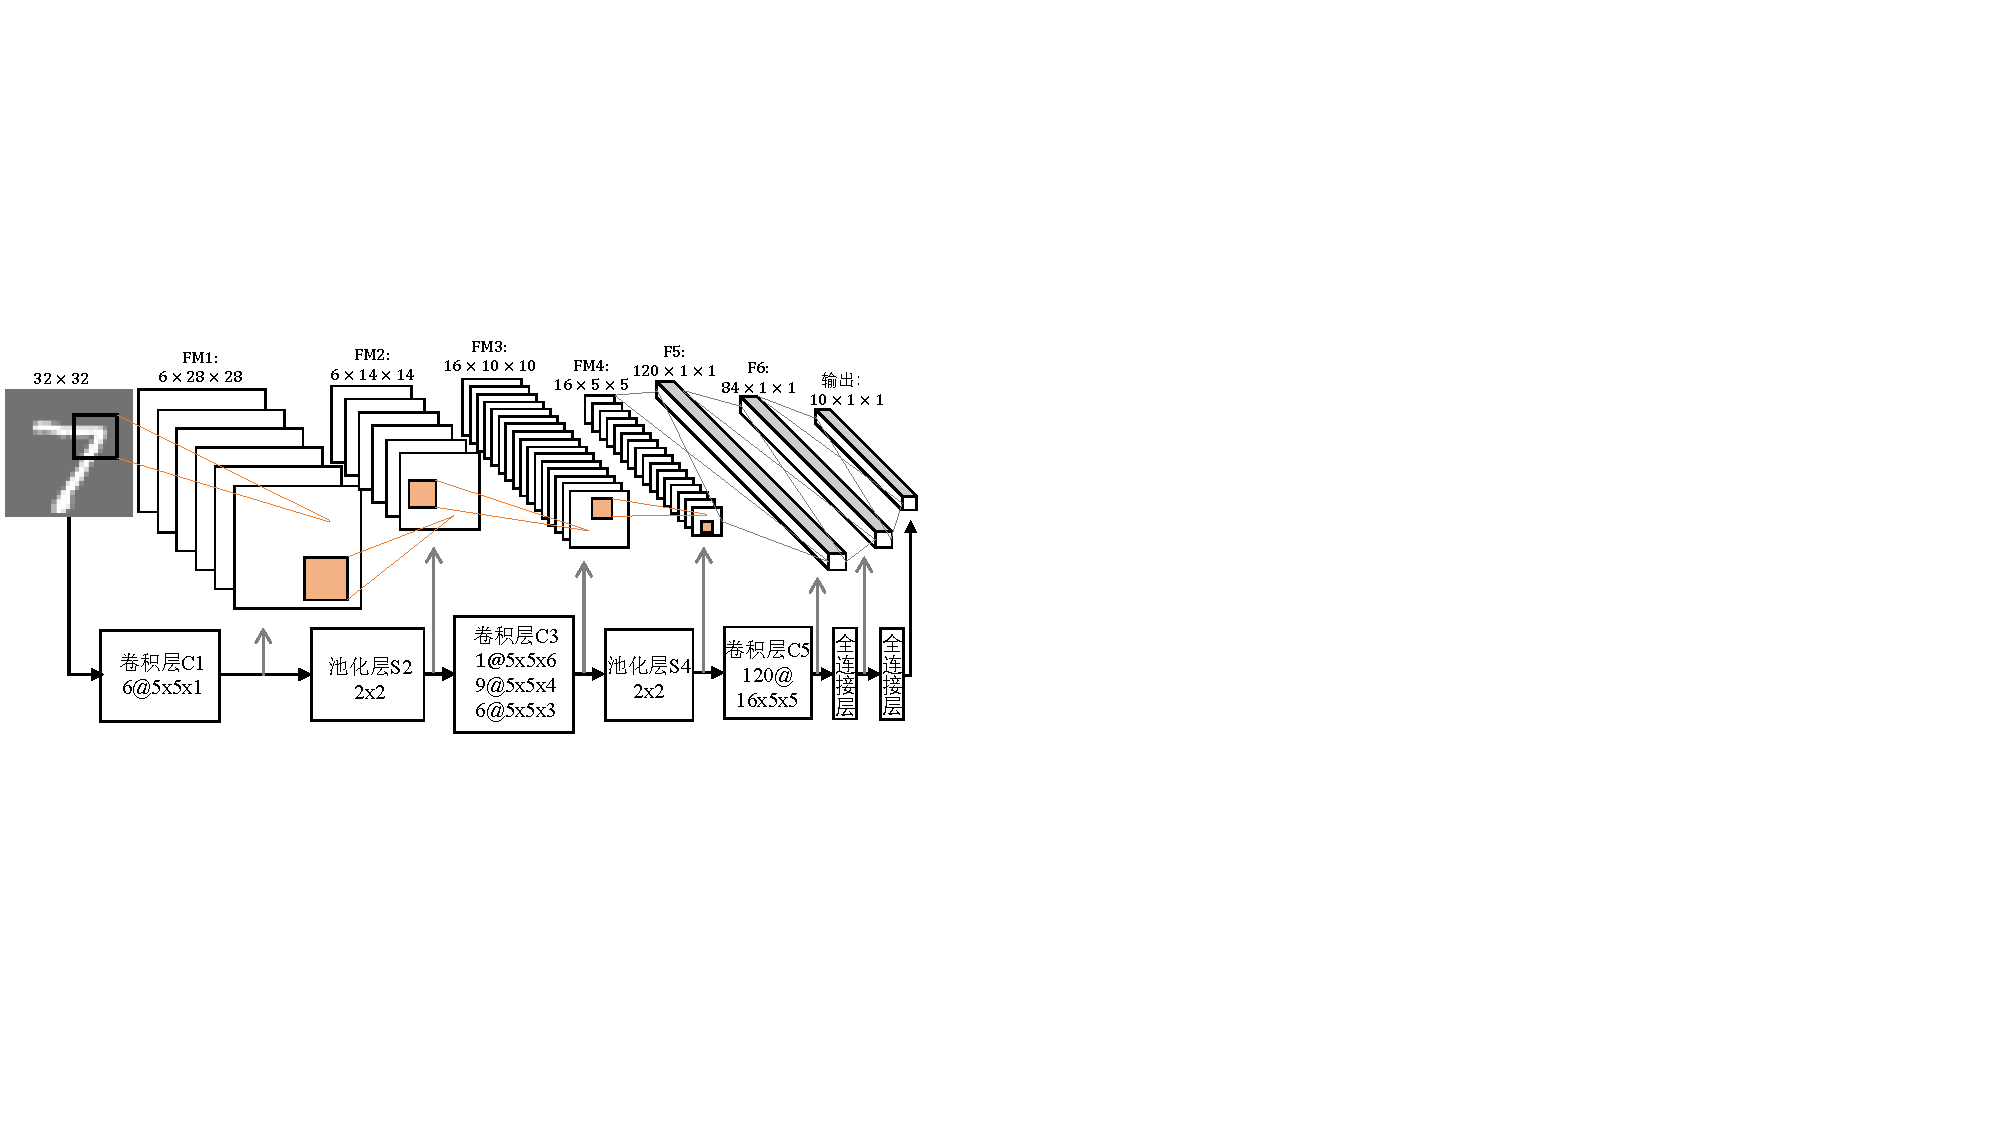
\includegraphics[scale=0.9]{Img/fig_2_lenet5.pdf}
    \bicaption{LeNet-5模型示意图}{Schematic diagram of the LeNet-5 model}
    \label{fig:2_lenet5}
\end{figure}
LeNet-5是最早的卷积神经网络模型之一,设计之初被用于手写数字识别任务。图\ref{fig:2_lenet5}展示了LeNet-5从输入图片到输出预测结果的模型工作简化图。LeNet-5共包含5层,包括两个卷积层(convolutional layer)C1、C3、C5,以及两个池化层(pooling layer)S2和S4。

{\sffamily 卷积层:}卷积层是CNN模型的核心模块,包含了整个模型的大部分参数。它可以对输入图像的局部区域进行加权求和从而得到图片的特征(feature)或特征图(feature map,FM),例如示例中经过卷积层得到的特征或特征图有FM1、FM3和F5。卷积层中卷积核(convolution kernel)大小和形状的选择能够影响卷积的效果。例如,图\ref{fig:2_lenet5}中卷积层C1中有6个$5 \times 5 \times 1$的卷积核,每个卷积核将图片中每个$5 \times 5$大小区域内的像素点加权求和得到输出特征图中的一个像素点,那么一个$32 \times 32$大小的图片经过卷积层C1后得到的特征图FM1的大小为$6 \times 28 \times 28$。经过卷积层后,图片的通道数可能会增加,图片的尺寸也可能变小。卷积层的设计可以很简单也可以非常的复杂,例如卷积层C3中包含了16个卷积核,其中各卷积核的尺寸为$5 \times 5$,但选取的特征图数量(图中包含6,4,3三种数量的差别)却各不相同。这说明卷积层的设计可以是非常灵活的,也因此对模型设计与研究人员的考验也是巨大的。

{\sffamily 池化层:}池化层一般也成为下采样层(subsampling layer),相当于一个过滤器,对图片或特征图执行降维操作,滤掉无用的像素点,帮助模型提取更高层次的特征。其原理是在输入特征图中一个局部区域内,按照选取最大值或计算平均值的方式为输出特征图增加一个新的像素点,也称最大池化(max pooling)和平均池化(average pooling)。例如图\ref{fig:2_lenet5}中的池化层S2的大小为$2 \times 2$,它在图片中对应区域内选取最大值或计算平均值后输出到特征图FM2中。区别于卷积层,池化层对输入特征图进行过滤像素时,一般不设置重叠区域,例如图中的池化层的尺寸和步长均为2,因此特征图经过池化层后特征图的尺寸变为原来的二分之一。

{\sffamily 全连接层:}全连接层(full connection layer)层中的每个神经元都连接着上一层的所有神经元。区别于卷积层和池化层将图片映射到隐层的特征空间中,而全连接层将隐层表示映射为图片的分布式特征表示,或经过非线性激活函数(一般采用softmax函数)得到样本的概率模型并预测样本的分类结果。例如图\ref{fig:2_lenet5}中最后的全连接层将图片特征F6映射为一个维度为10的向量中,每个维度的取值为0到1,代表着预测为0到9每个值的概率。

虽然LeNet-5的结构简单,但依旧展现了卷积神经网络能够学习并表征图片信息的能力。层数更深,网络结构更复杂,以及采用了更多新技术的新一代卷积神经网络能够表征更复杂的图像信息。在融合视觉信息的自然语言处理任务中,因文本输入与图片输入很难在一个模型中同时支持,因此通常采用特征融合的方式支持多模态输入。从一般的卷积神经网络的模型结构可以看到,选取图片特征的选择可以有很多种。例如图\ref{fig:2_lenet5}中FM4的尺寸为$16 \times 5 \times 5$,其中,在$5 \times 5$的特征图内仍保留着与源图片中的区域对应关系。因此FM4可看作是由$5 \times 5$个维度为16的特征组合而成,每个16维的特征表征了图片中对应的区域。这种保留了图片内局部空间信息的特征图一般称为栅格特征(grid feature)或局部特征(local feature)。在融合图片信息的神经机器翻译方法中,栅格特征一般可以作为图片输入序列输入到翻译模型中,通过注意力机制能够动态地关注到栅格特征中保留的局部空间信息。利用平均池化将栅格特征所代表的多个视觉特征融合为一个视觉特征,称作全局特征(global feature)。全局特征表征了图片的全局信息,通常可以用于初始化循环神经网络,或作为词向量等方式输入到神经机器翻译模型中。

% 要强调栅格信息保留了位置信息
% 这里最好直接举ResNet的例子,可以直接将残差连接的引入到现有机器翻译模型中

\subsection{目标检测方法}
%方法背景介绍
目标检测是计算机视觉领域中一个应用范围非常广的任务,其目的是在图像或视频中自动地定位并识别出特定的视觉目标,从而满足对视觉目标的筛选、分类、追踪等需求。早期的目标检测算法需要手工设计特征和分类器来实现物体检测,并且运行速度较慢。随着深度学习的发展,目标检测算法开始采用卷积神经网络作为基础模型实现对视觉目标的检测,并取得了很好的性能与速度。对于融合图片信息的神经机器翻译任务,目标检测同样是非常重要的应用手段之一。与卷积神经网络能够提供图片的全局特征和栅格特征相比,目标检测的结果能够直接将图片中最有价值的前景信息提供给翻译模型。并且,每个视觉目标都能够提供排除与视觉目标不相关的更集中的视觉信息。

根据各算法特点以及工作方式,可以将目前常用的目标检测算法可以分为三类:两阶段法、一阶段法、语义目标提取法(visual grounding)。其中两阶段法和一阶段法提取给定图片中的所有类别可知的目标,并将提取出的目标分到相应的类别。语义目标提取法是根据语义信息提取相应的视觉目标,因此可以与前两者区分开。


\begin{figure}[!htbp]
    \centering
    \begin{subfigure}{\textwidth}
      \centering{
      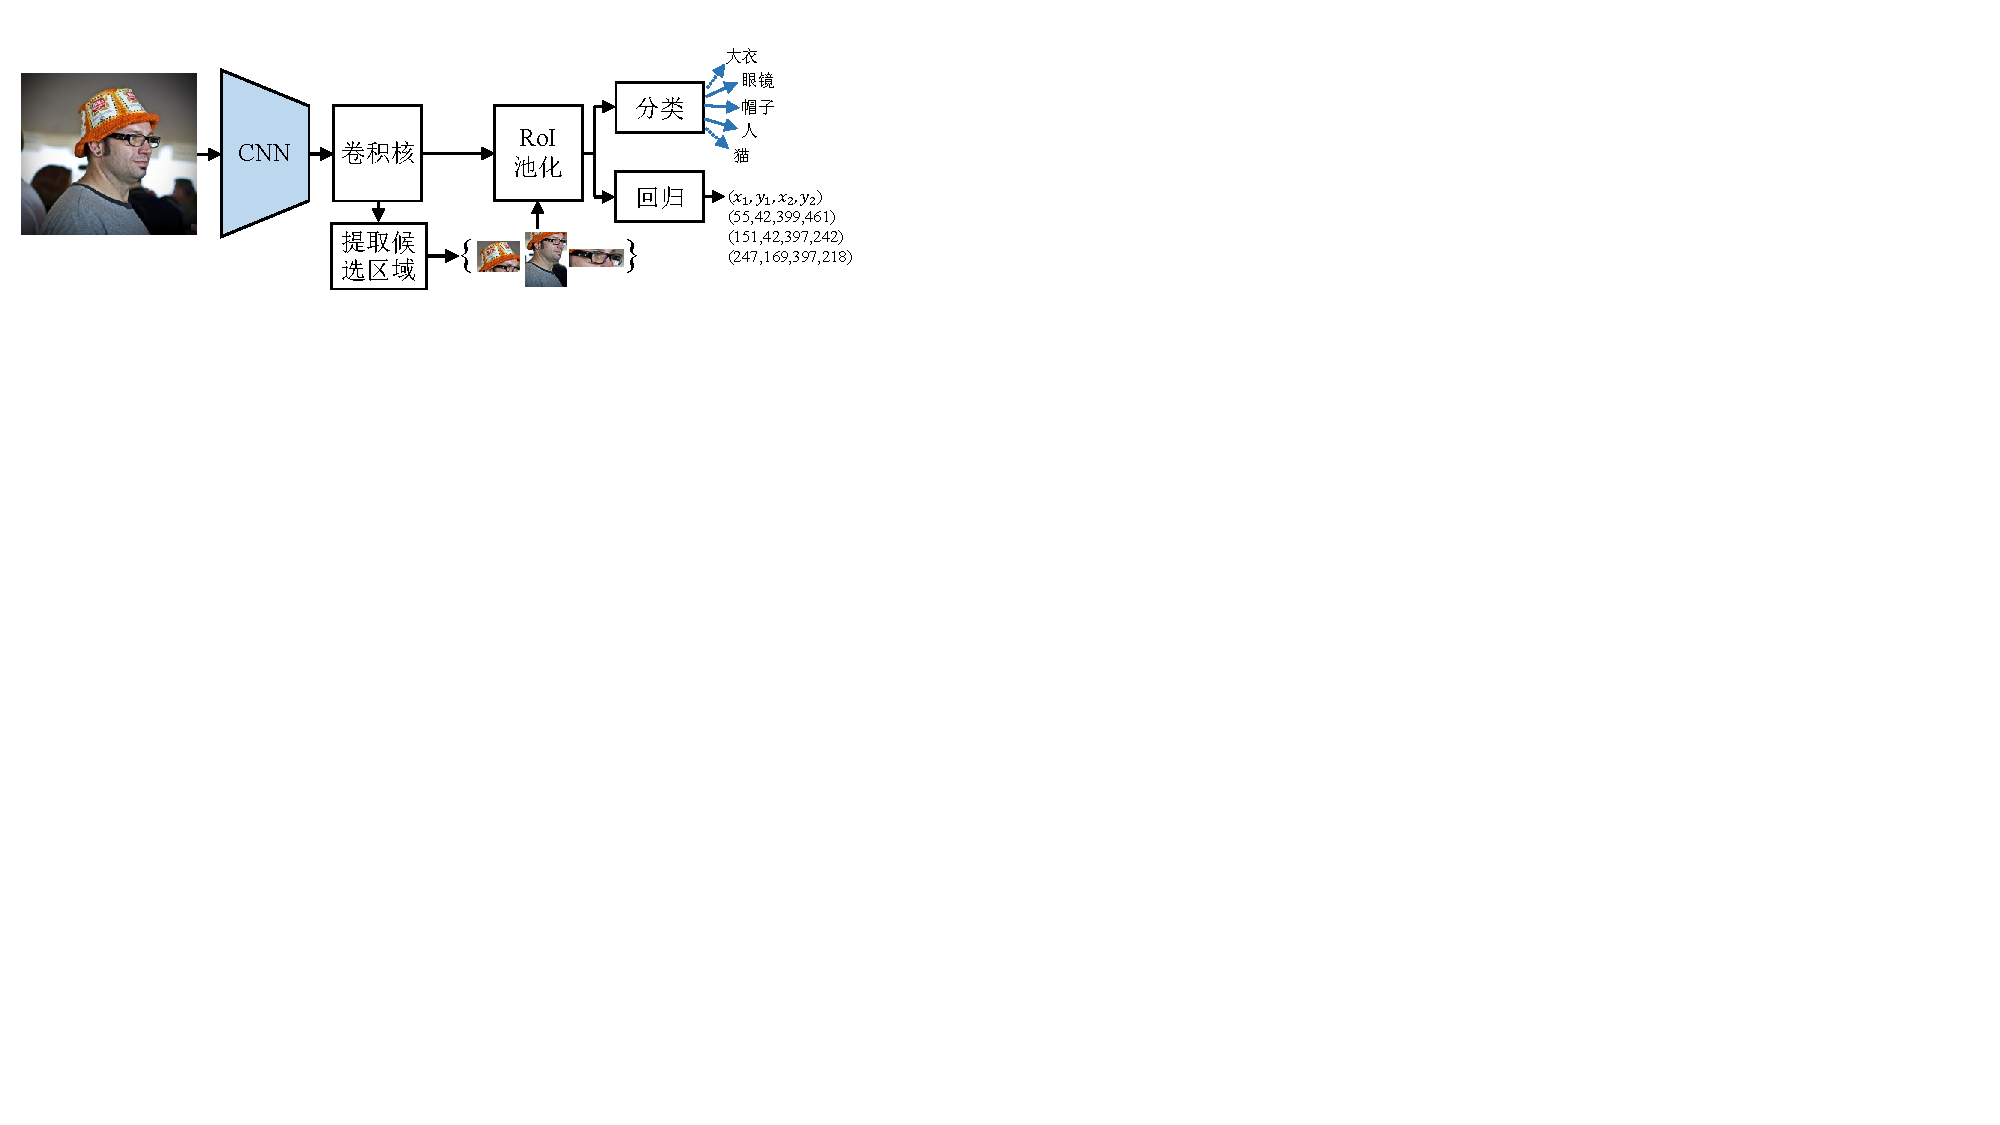
\includegraphics[scale=1.0]{Img/fig_2_rcnn.pdf}
      \caption{两阶段目标检测算法简图}
      \label{fig:2_rcnn}}
    \end{subfigure}%
    \\% line break
    \begin{subfigure}[b]{\textwidth}
      \centering
      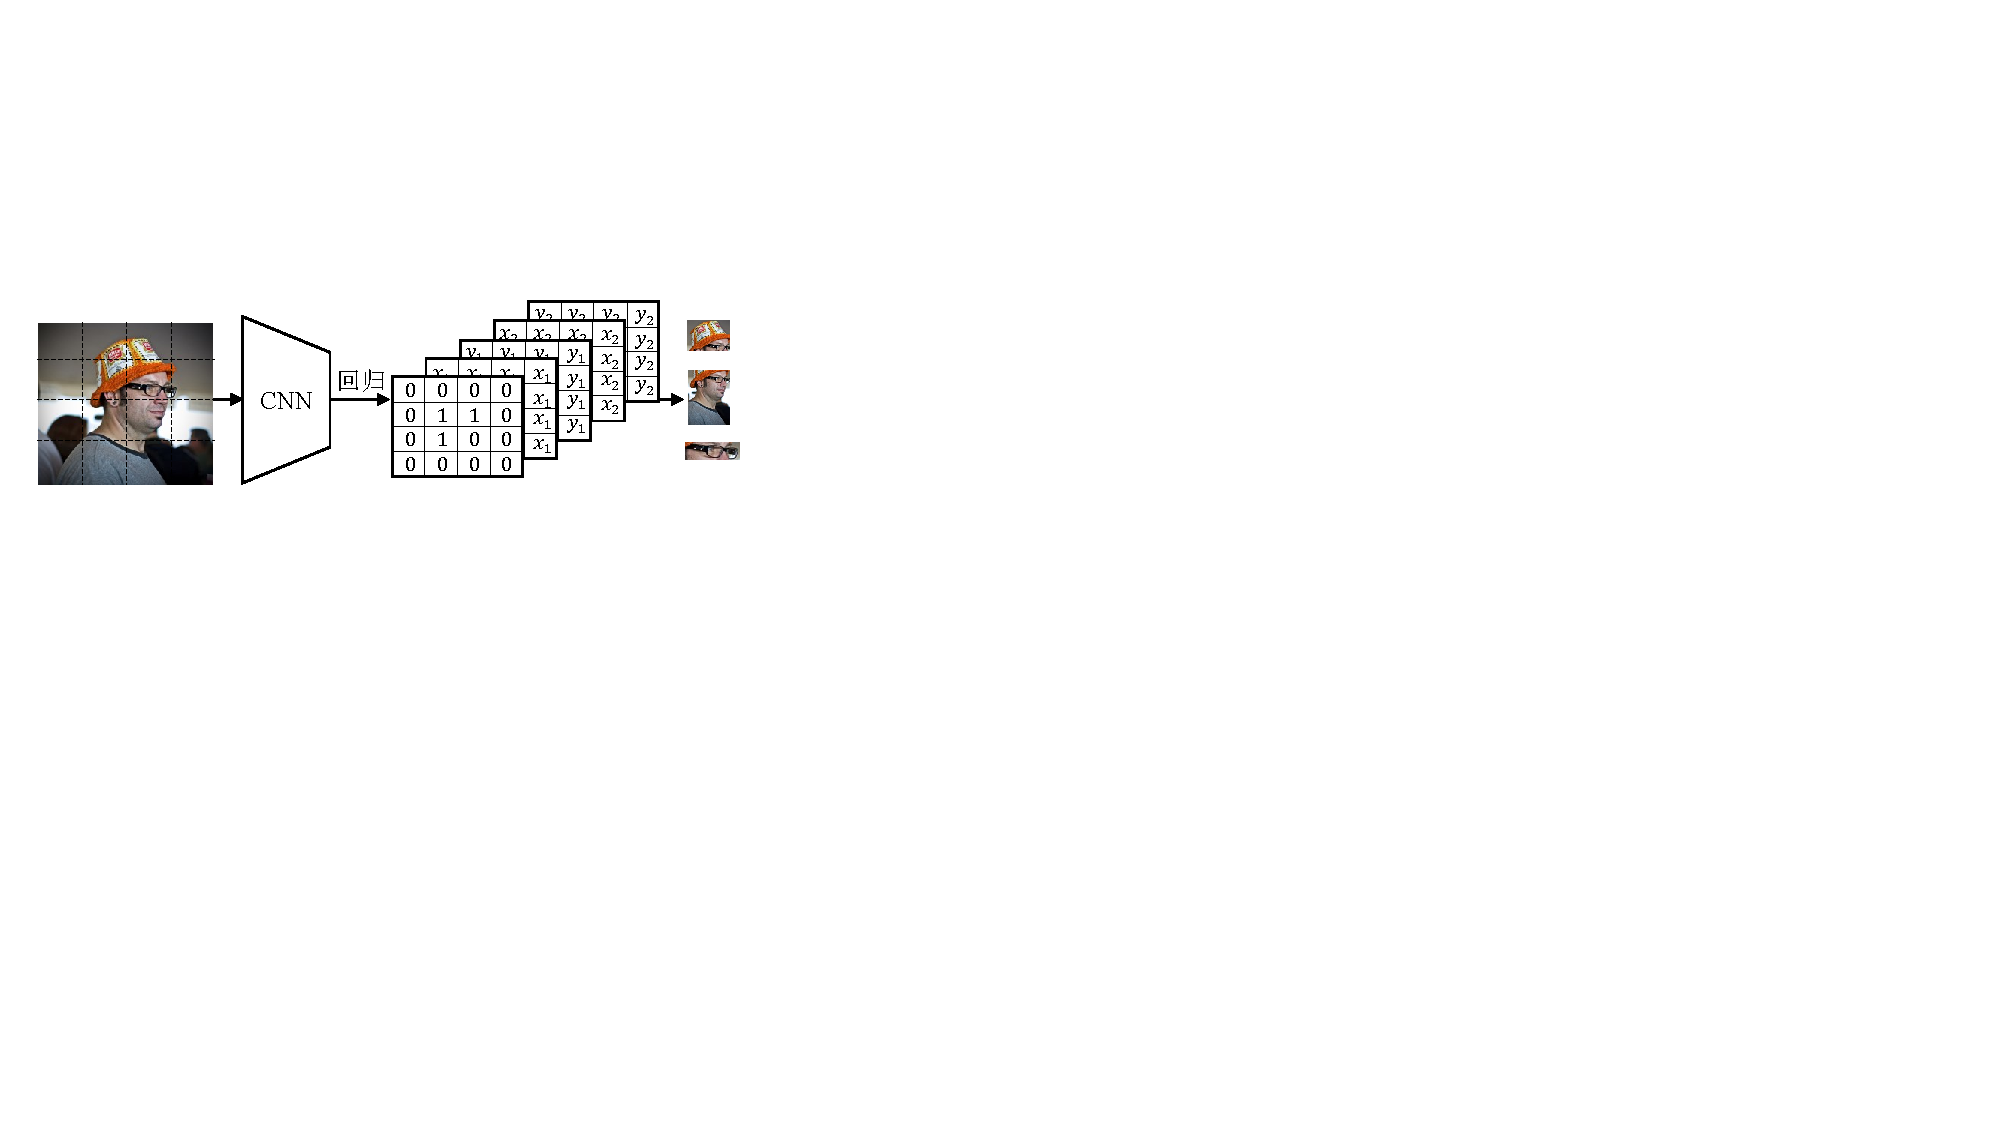
\includegraphics[scale=1.0]{Img/fig_2_yolo.pdf}
      \caption{一阶段目标检测算法简图}
      \label{fig:2_yolo}
    \end{subfigure}
    \\% line break
    \begin{subfigure}[b]{\textwidth}
      \centering
      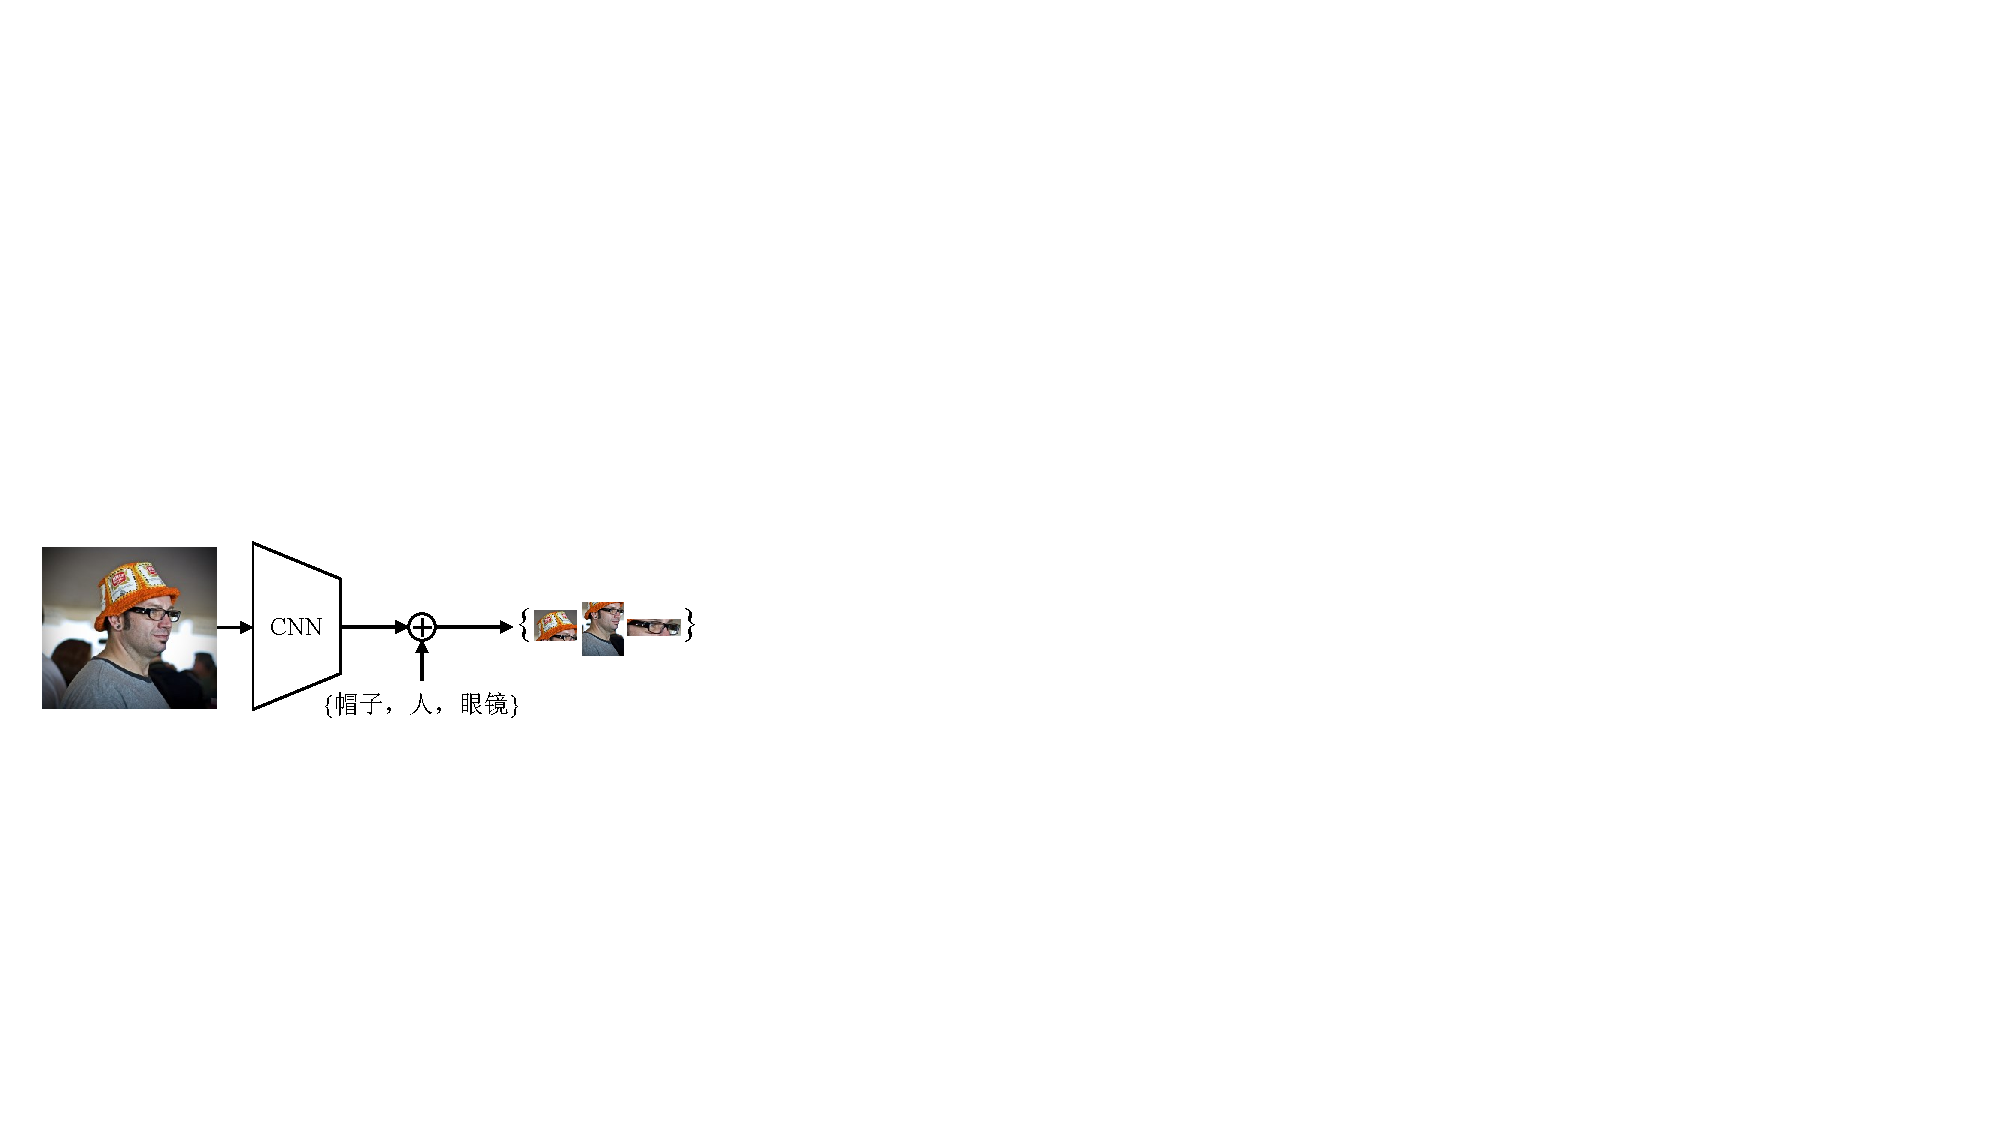
\includegraphics[scale=1.0]{Img/fig_2_visual_grounding.pdf}
      \caption{语义目标提取法简图}
      \label{fig:2_visual_grounding}
    \end{subfigure}%
    \bicaption{目标检测算法示意图}{Schematic diagram of object detection algorithm}
    \label{fig:2_object_detection}
\end{figure}
{\sffamily 两阶段法}

两阶段法的代表方法有R-CNN(region-based convolutional neural networks)、Fast R-CNN以及Faster R-CNN。因这类算法在目标检测过程中分为提取候选区域(region proposal)和“特征提取与分类回归”两步

{\sffamily 一阶段法}

{\sffamily 语义目标提取法}

%方法介绍

%在ImgNMT中的应用

对于跨模态信息融合,目标检测依旧是非常重要的应用手段之一。与卷积神经网络相比,目标检测的结果能够直接将图片中那些信息量最大的目标直接提供给翻译模型,而提取出的视觉目标所包含的信息也更集中。目标检测的结果可以分为两种,一种是检测结果与文本不建立关系,此时目标检测方法输出的多个视觉目标结果可以视为视觉目标序列输入到以序列建模擅长的自然语言处理任务的模型中。另一种是通过文本语义进行视觉目标检测,这种方式能够对齐文本与视觉目标,更方便在翻译中使用。
% 目标检测要给出区域,和分类
% 最初的设定,扫描图片中的所有框
% R-CNN:two-stage,ROI->feature extraction for ROI->SVM->位置精修
%      R-CNN-> Fast R-CNN -> Faster R-CNN
% Yolo v0-5: one-stage (you only look once)(regression)
%      v0: 遍历所有“框” -》 输出(c,x,y,w,h) 其中c为confidence,label为(1,x*,y*,w*,h*)
%      v1:检测多个目标,将img划分为多个区域,(c,x,y,w,h,one-hot)*N
% visual grounding

\subsection{视觉Transformer}
%这里和前面呼应以下,前面是CV推动着NLP的发展,这里则反过来,NLP推动CV

%预示着大模型的融合

%与CNN相同同样可以做backbone,做目标检测以及图片分类

% 结尾说以下那几篇文章说过使用哪种CNN-backbone带来的差别并不大
% 2.4 MMT
\section{多模态神经机器翻译}
\subsection{图片信息辅助式神经机器翻译}
得益于神经网络方法的快速发展,自然语言文本与图片的信息融合成为了可能。融入图片信息的机器翻译的研究历程也紧随着纯文本的神经机器翻译的脚步而发展。然而,相关研究则最早起源于图像描述生成任务。有部分学者将文本作为一个外源信息来辅助图片描述的生成,但这种方式的本质则是在翻译任务中融入视觉信息。2016年WMT将多模态机器翻译引入作为共享任务后,MMT受到了广泛的关注。在之后的WMT17和WMT18,MMT任务延续并奠定了在机器翻译中融合图片信息作为多模态机器翻译研究的主要范式。

%平行翻译句一般具有良好的对齐特性,这使得融入的外源信息仅用于辅助少数具有歧义、信息不完整以及训练不充分等问题的句子的翻译。该特性也成为了展开相关研究道路上的一大难点。
融合图片信息的神经机器翻译任务主要采用的是平行翻译句对加图片三元组形式的数据,即一张图片对应一句描述和一句翻译。大部分相关研究需要对神经机器翻译模型进行适当的修改,以适应图片的输入。模型中输入的图片可用于辅助优化翻译过程中源语言的语义表示,或为解码过程增加辅助外源信息。本文将这种在翻译过程中以源端文本作为信息主体,输入图片用于语义信息强化的方法称为图片信息辅助式神经机器翻译。可根据图片信息融合到翻译模型中的方式将这种方法分为三类:融合图片全局信息、融合图片局部动态信息以及融合图片视觉目标信息。这些三种图片信息以视觉特征为载体输入到翻译模型中,视觉特征则是从预训练的卷积神经网络中提取得到。不同的提取方式所包含的语义信息的粒度和特征维度有所不同。将这些不同形式的视觉特征整合到NMT模型后,模型进行跨模态语义融合的难易程度则取决于模型设计的合理性。

\subsubsection{融合图片全局信息的神经机器翻译}

\cite{18_DBLP:conf/emnlp/CalixtoL17}
\cite{19_DBLP:conf/acl/CalixtoRA19}
\cite{20_DBLP:conf/acl/WuKBLK20}


\subsubsection{融合图片局部动态信息的神经机器翻译}

\subsubsection{融合图片视觉目标信息的神经机器翻译}

\subsection{图片信息增强式神经机器翻译}

\subsection{基于图片搜索的神经机器翻译}

\subsection{跨模态无监督神经机器翻译}
%\section{图片信息辅助式神经机器翻译}
得益于神经网络方法的快速发展,自然语言文本与图片的信息融合成为了可能。融入图片信息的机器翻译的研究历程也紧随着纯文本的神经机器翻译的脚步而发展。然而,相关研究则最早起源于图像描述生成任务。有部分学者将文本作为一个外源信息来辅助图片描述的生成,但这种方式的本质则是在翻译任务中融入视觉信息。2016年WMT将多模态机器翻译引入作为共享任务后,MMT受到了广泛的关注。在之后的WMT17和WMT18,MMT任务延续并奠定了在机器翻译中融合图片信息作为多模态机器翻译研究的主要范式。

%平行翻译句一般具有良好的对齐特性,这使得融入的外源信息仅用于辅助少数具有歧义、信息不完整以及训练不充分等问题的句子的翻译。该特性也成为了展开相关研究道路上的一大难点。
融合图片信息的神经机器翻译任务主要采用的是平行翻译句对加图片三元组形式的数据,即一张图片对应一句描述和一句翻译。大部分相关研究需要对神经机器翻译模型进行适当的修改,以适应图片的输入。模型中输入的图片可用于辅助优化翻译过程中源语言的语义表示,或为解码过程增加辅助外源信息。本文将这种在翻译过程中以源端文本作为信息主体,输入图片用于语义信息强化的方法称为图片信息辅助式神经机器翻译。可根据图片信息融合到翻译模型中的方式将这种方法分为三类:融合图片全局信息、融合图片局部动态信息以及融合图片视觉目标信息。这些三种图片信息以视觉特征为载体输入到翻译模型中,视觉特征则是从预训练的卷积神经网络中提取得到。不同的提取方式所包含的语义信息的粒度和特征维度有所不同。将这些不同形式的视觉特征整合到NMT模型后,模型进行跨模态语义融合的难易程度则取决于模型设计的合理性。

\subsection{融合图片全局信息的神经机器翻译}

\cite{18_DBLP:conf/emnlp/CalixtoL17}
\cite{19_DBLP:conf/acl/CalixtoRA19}
\cite{20_DBLP:conf/acl/WuKBLK20}


\subsection{融合图片局部动态信息的神经机器翻译}

\subsection{融合图片视觉目标信息的神经机器翻译}



%% 2.4 visual enhanced MMT
%\section{图片信息增强式神经机器翻译}
%% 2.5 retrieval-based MMT
%\section{基于图片搜索的神经机器翻译}





\section{本文研究思路}
% 还要几篇分析性质的工作
% MMT的演变与拥有的优势
% MMT现有存在的问题
从基于循环神经网络的RNMT,到目前广泛采用的Transformer,研究者们致力于将图片中的视觉信息以各种方式融合到翻译过程中,从而提升机器翻译的质量。这是因为,相比于纯文本,图片中往往包含更完整、更细节以及更丰富的语义信息。然而,相比于纯文本翻译利用端到端模型就可以学习到跨语言的表示与生成,融入图片信息的神经机器翻译并不是简单地将图片输入到模型中就能够将跨模态的信息进行融合并利用。

得益于不同模态的信息在神经网络方法中普遍以分布式向量表示的形式呈现,在神经翻译模型中实现跨模态信息融合具有很强的优势:1)能够直接从数据中学习数据特征,不需要人为的特征设计;2)采用成熟的神经翻译模型作为主框架,采用预训练的卷积神经网络用于图片编码,跨模态信息融合可以在现有模型基础上进行改进;3)图片作为上下文信息的表示方法与融合方式,和一般的文档上下文或视频上下文类似,相应的模型方法有很强的泛化复用性;4)解决歧义词或语义不完整等文本中出现信息缺失的问题。

% 本文索要解决的问题:三篇文章
然而,已有方法同样存在一些问题,例如翻译质量的提升不稳定,图片信息的作用方式不明确,翻译模型对视觉信息不敏感等问题。尽管当前广泛应用的神经翻译模型与计算机视觉基础模型为跨模态信息融合提供了极大的便利,依旧难以针对不同跨模态信息需求的文本翻译数据设计统一的模型方案。为此,本文尝试回答三个问题:
\begin{itemize}
    % 输入图片不一定带来提升
    \item {\sffamily 翻译质量提升不稳定}。文献\cite{21_dutta-chowdhury-elliott-2019-understanding,22_li-etal-2021-vision,20_wu-etal-2021-good}的实验表明,相比于纯文本神经翻译,输入图片信息后的翻译模型的翻译准确率并没有得到明显的提升,有些甚至会低于纯文本翻译。这说明在一般的翻译模型中,将图片中的视觉信息与文本信息的融合并不是一个必然的过程。如何使融合图片信息的神经机器翻译获得有效的翻译准确率的提升?
    % 隐含式方法的弊端
    \item {\sffamily 图片信息作用方式不明确}。尽管已有很多模型方法表明输入图片信息能够为翻译质量带来提升,然而图片信息的作用方式并不明确。例如,歧义词问题是否得到解决?语义不完整的句子是否得到补全?亦或是在其它不得而知的方面为翻译带来的增益?如何以更明确的方式将视觉信息作用到神经翻译中?
    % 输入噪音可能比输入图片带来的提升更多
    \item {\sffamily 翻译模型对视觉信息不敏感}。文献\cite{23_elliott-2018-adversarial}将与文本内容不一致的图片输入到翻译模型中来测试模型翻译准确率的提升是否来自于图片中的视觉信息,实验结果显示大部分模型可以从错误的图像中获得同样或相近的翻译准确率的提升。文献\cite{20_wu-etal-2021-good}认为输入图片与输入早已的作用相似,是正则化作用而非视觉信息为模型带来的翻译准确率的提升。如何使翻译模型对输入图片信息敏感?
\end{itemize}

为此,本文围绕融合图片信息的神经机器翻译方法研究,从改进模型的训练方式、图片的输入方式、视觉信息的作用方式等方面展开研究工作:
\begin{itemize}
    % 翻译质量提升不稳定,作用方式不明确
    \item {\sffamily 基于跨模态文本重构的神经机器翻译:}为解决图片信息作用方式不明确的问题,改变了图片的输入方式,使用图片的视觉目标特征以替换的方式作用到名词短语或名词两种粒度上,用于重构完整的文本。然后改变了模型的训练方式,以多任务训练的方式,利用多模态重构任务优化神经机器翻译模型的表示能力,从而提升翻译的准确率,得到具有稳定提升翻译质量能力的神经翻译模型。第3章将介绍我们提出的基于跨模态文本重构的神经机器翻译方法。
    % 翻译质量提升不稳定,作用方式不明确
    \item {\sffamily 基于双向跨模态实体重构的神经机器翻译:}在上一部分工作的基础上,以更明确的方式,针对实体词和视觉实体,实现双向跨模态实体重构。区别于重构完整的文本,针对实体词即可得到较好的模型结果。第4章介绍我们提出的基于双向跨模态实体重构的神经机器翻译方法。
    % 翻译质量提升不稳定,对视觉信息不敏感
    \item {\sffamily 基于图文对比对抗训练的神经机器翻译:}在训练融合图片信息的神经翻译模型的同时,采用对比学习方法学习译文与多模态输入的联合语义表示空间。为了解决模型对视觉信息不敏感的问题,在对比学习的负样本集中加入图文不一致的对抗样本。通过提升翻译模型区分输入图片正确与否的能力,强迫模型将图片中的视觉信息融合到文本表示中,从而强化源端文本的特征表示,实现翻译准确率的提升。第5章将介绍我们提出的基于图文对比对抗训练的神经机器翻译方法。
\end{itemize}
%(在这里提到模型对视觉信息不敏感的问题,然后循序渐进讲为什么我们的研究以增强式为主,后又如何补充辅助式)

\section{本章小结}
本章介绍了与融合图片信息的神经机器翻译相关的国内外研究,其中包括神经机器翻译主流模型的发展过程。然后主要介绍了在神经翻译模型中融合图片信息的主流方法,以及各类方法所具备的特点。本章分析了现有融合图片信息的神经机器翻译方法的缺陷,简要地说明了相应的解决办法,以及针对这些问题本文的一些应对思路。这些内容与本文的研究内容息息相关,在后面的章节中,本文将针对如何将图片中的视觉信息融合到神经翻译模型中给出相应的解决方案。

